%---------- Inleiding ---------------------------------------------------------

\section{Introductie} % The \section*{} command stops section numbering
\label{sec:introductie}


De keuze voor cross platform applicaties wordt de dag van vandaag steeds aantrekkelijker. Dit kan onder andere verklaard worden door de financiële voordelen ten opzichte van native applicaties, meer specifiek op vlak van de impact op het ontwikkelingsbudget van bedrijven.  Cross platform applicaties worden al heel lang gepromoot als zijnde 'beter' dan native applicaties. Deze cross platform applicaties zijn sneller te ontwikkelen en vereisen minder lijnen code. De slogan “Write once, run anywhere” van Sun Microsystems \autocite{Oracle} wordt vaak gebruikt om het grote voordeel van cross platform applicaties aan te duiden, dit duidt op het idee dat grote delen van de code kunnen gebruikt worden voor verschillende besturingssystemen. De duurdere native applicaties hebben echter nog steeds een aantal voordelen ten opzichte van de cross platform applicaties, aangezien deze specifiek geschreven zijn voor het gekozen besturingssysteem zoals bijvoorbeeld voor Android of iOS. De meeste reeds bestaande cross-platform frameworks, zoals Flutter, delen de user interface van de applicatie over de verschillende besturingssystemen. Dit zorgt voor een applicatie die voor geen enkel van de gekozen besturingssysteem perfect zal zijn, aangezien hierbij dan geen gebruik kan gemaakt worden van de specifieke frameworks voor dat specifieke besturingssysteem. Kotlin Multiplatform Mobile (KMM) gooit het concept van cross platform over een andere boeg en werkt met een gedeelde businesslogica in plaats van een gedeelde user interface. De applicaties worden dus elk afgewerkt met een native user interface. De opzet van deze bachelorproef is na te gaan of native applicatieontwikkeling voor Android en iOS apparaten nog steeds de beste keuze is of KMM een sneller en efficiënter alternatief kan vormen binnen het huidige beeld van applicatieontwikkeling. Om dit te onderzoeken zijn er bepaalde testcriteria opgesteld. Deze testcriteria zijn: het aantal lijnen code, de kostprijs, de ontwikkeltijd, de compileersnelheid, de voetafdruk en de uitbreidingsmogelijkheden van de applicaties.  Aan de hand hiervan kan besloten worden of de KMM-applicaties een beter alternatief kunnen vormen voor native applicaties. Daarnaast zal ook de vraag gesteld worden of het huidige beeld van de SWOT-analyse voor cross-platform applicaties ook toepasbaar is voor KMM-applicaties, indien niet zal gekeken worden hoe deze dient aangepast te worden. 

%---------- Stand van zaken ---------------------------------------------------

\section{State-of-the-art}
\label{sec:state-of-the-art}


\subsection{Kotlin}
\label{sec:kotlin}
In juli 2011 kwam JetBrains, de maker van onder andere IntelliJ IDEA, naar buiten met een nieuw project genaamd Kotlin.\autocite{Jemerov2011} Kotlin is een algemene, cross-platform en statische taal met type-inferentie. \autocite{Oliveira2020} Hierbij verwijst de term algemene naar het feit dat Kotlin is ontwikkeld is voor allerlei verschillende types van software en in verschillende situaties kan gebruikt worden. Cross-platform gaat over het gegeven dat software kan bestaan in verschillende versies op meer dan één platform. Ook is er vernoemd dat Kotlin statische typering gebruikt als taal, dit komt neer op het feit dat Kotlin de types van de objecten zal controleren tijdens het compileren van de code en niet tijdens het uitvoeren. Andere talen die dezelfde strategie volgen zijn Java en C. Alsook zal Kotlin gebruik maken van type-inferentie, hiermee zal de taal zelf onderscheid kunnen maken tussen datatypes van bepaalde expressies. 

\subsection{Cross-platform en native}
\label{sec:cross-platform_en_native}

Allereerst moet de omschrijving van een platform besproken worden, een platform zal meestal een bepaalde programmeertaal, besturingssysteem of bepaalde hardware beschrijven. Dit kan ook een combinatie van meerdere zijn.\autocite{Bishop2006} Hiervan zijn enkele voorbeelden Java SE 15, hierbij wordt de taal bedoeld als platform. Een voorbeeld van een platform als besturingssysteem is bijvoorbeeld Windows 10 of MacOS Big Sur. Een voorbeeld hardware als platform is bijvoorbeeld een Intel of AMD processor. Uiteindelijk kan er ook gezegd worden dat een computer met als besturingssysteem Windows 10 en een laatste generatie Intel processor ook een specifiek platform is.
\\ \\
Eens de term platform duidelijker is, kan er makkelijker omschreven worden wat precies een cross-platform applicatie is en wat een native applicatie is. Een cross-platform applicatie is zoals de naam het al zegt een applicatie die op meerdere platformen zal werken. De software zal dus licht verschillende versies hebben die op hun beurt op allerlei verschillende platformen zullen werken. Native applicaties daarentegen zullen zich toespitsen op één bepaald platform.
\\ \\
Verder wordt er SWOT-analyse bekeken voor cross-platform applicaties. Deze sterkte-zwakteanalyse zal bekijken wat de sterktes en zwaktes zijn maar ook een beeld schetsen van de kansen en bedreigingen. Hiermee kunnen we een beeld schetsen wat de huidige positie is van cross-platform applicaties binnen de huidige markt. Uit onderzoek van Tommi Nivanaho naar cross-platform applicaties met React Native zijn een aantal factoren naar voor gekomen.\autocite{Nivanaho2019} Hier moet wel rekening gehouden worden met het feit dat sommige factoren niet toepasbaar zijn op alle cross-platform SDK’s en toolkits. Hieronder een overzicht van enkele punten uit de studie toepasbaar zijn op cross-platform applicaties in het algemeen.
\\
\begin{itemize}
\item Sterktes of Strengths
\begin{itemize}
\item Sneller te ontwikkelen
\item Kostenbesparend
\item De applicatie ondersteunt meerdere platformen tegelijkertijd
\end{itemize}
\item Zwaktes of Weaknesses
\begin{itemize}
\item Nog steeds nood aan native code per platform
\item Upgrades kunnen omslachtiger zijn
\end{itemize}
\item Kansen of Opportunities
\begin{itemize}
\item Snelle ontwikkeling voor meerdere platformen tegelijkertijd
\item Native applicaties kunnen relatief vlot omgevormd worden naar cross-platform applicaties
\end{itemize}
\item Bedreigingen of Threats
\begin{itemize}
\item Updates aan het gekozen cross-platform systeem kunnen de reeds geschreven applicaties onbruikbaar maken
\end{itemize}
\end{itemize}

\subsection{Kotlin Multiplatform}
\label{sec:kotlin_multiplatform}
Kotlin Multiplatform is de nieuwe cross platform software development kit (SDK) van JetBrains. Ook werd een SDK uitgebracht specifiek gericht op de mobiele toestellen namelijk Kotlin Multiplatform Mobile (KMM). Kotlin Multiplatform werd voor het eerst verwerkt in Kotlin 1.2 in november 2017 als experimentele functie.\autocite{Jemerov2017} 
Ondertussen heeft de ontwikkeling van KMM niet stil gestaan en is in augustus 2020 de alpha versie van deze SDK uitgebracht voor het grote publiek.\autocite{Petrova2020} In november 2020 werd de 0.2.0 versie uitgebracht, deze is verwerkt in Kotlin 1.4.20.\autocite{JetBrains2020} Enkele delen van deze SDK en bijhorende componenten zijn nog steeds in de experimentele fase van ontwikkeling, maar JetBrains geeft aan dat het nu al een ideaal moment is om deze software te testen.\autocite{Petrova2020} De community achter KMM en het open source verhaal spelen hier een grote rol en zullen ook zorgen voor een snellere ontwikkeling van deze software. Bedrijven kunnen dus momenteel al experimenteel aan de slag met deze nieuwe software en voorbeelden van enkele bedrijven die de stap al hebben gezet naar KMM zijn onder andere Netflix, VMware en Autodesk.\autocite{KotlinKMMCaseStudies}


\subsection{Kotlin Multiplatform versus  alternatieven}
\label{sec:kotlin_multiplatform_versus_alternatieven}
Kotlin Multiplatform (KM) zal het concept van cross-platform anders aanpakken dan andere alternatieven op de markt vandaag. Hierbij zit het verschil vooral in welke code van de applicatie zal gedeeld worden tussen de verschillende platformen. In de Kotlin documentatie staat beschreven hoe bepaalde delen van de code correct kunnen gedeeld worden tussen verschillende platformen. KM zal anders dan alternatieven de business logica delen tussen de verschillende platformen.\autocite{Kotlin2021} Hierbij wordt ook vermeld dat men enkel de business logica moet delen die gebruikt kan worden op alle platformen. 

\begin{figure}
    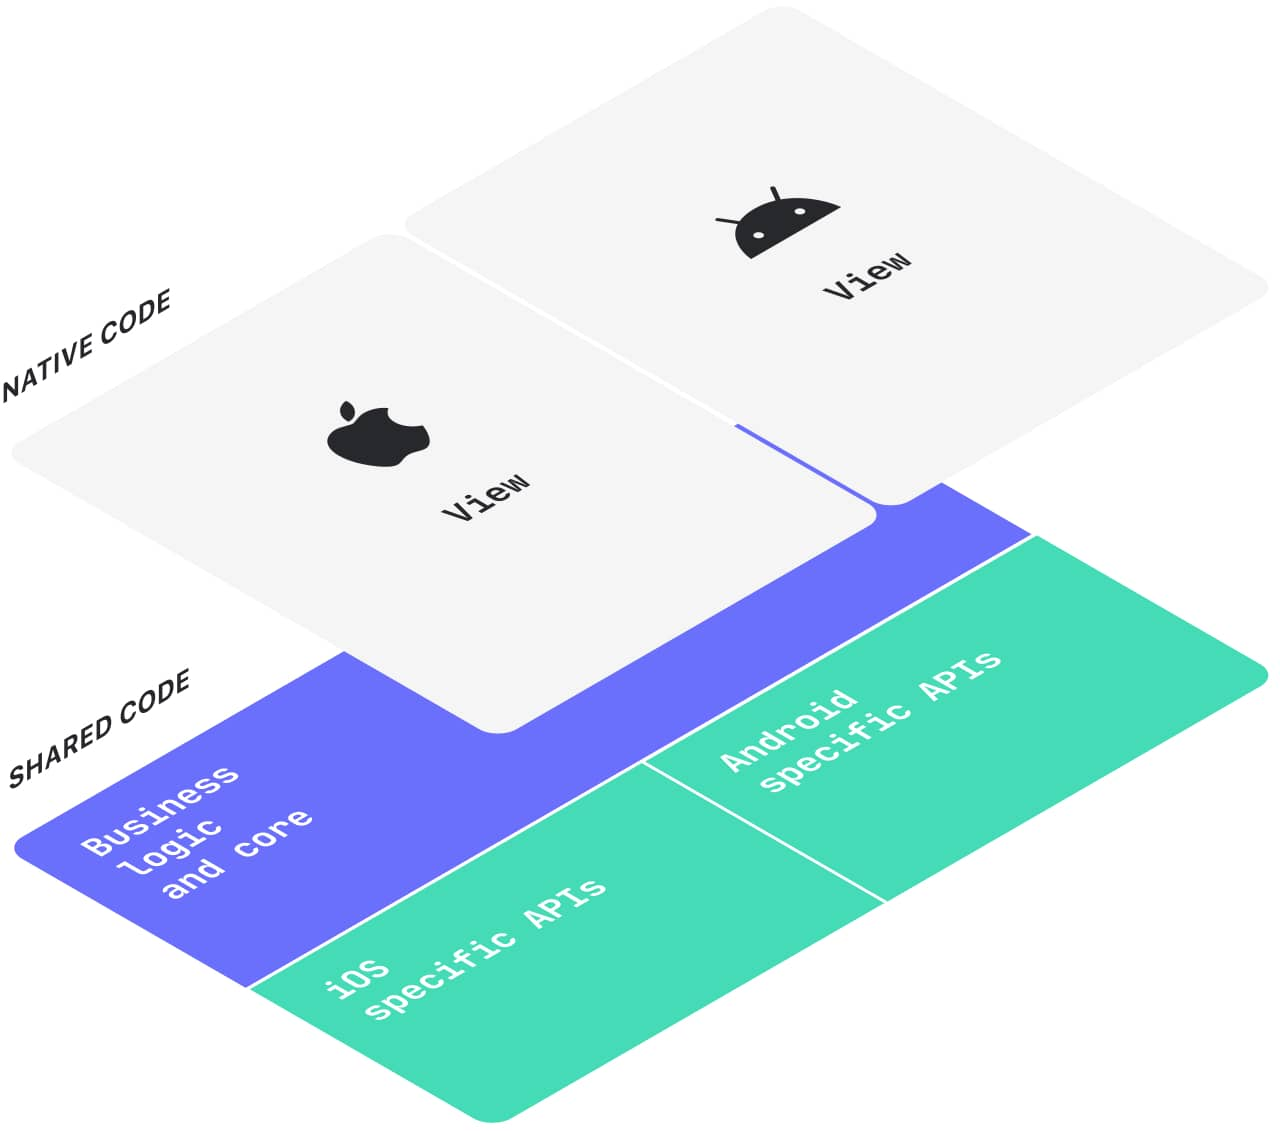
\includegraphics[width=\linewidth]{kmm.jpg}
    \caption{Grafische voorstelling Kotlin Multiplatform Mobile \autocite{KotlinKMM}}
    \label{fig:kmm}
\end{figure}

Figuur \ref{fig:kmm} geeft een goed algemeen beeld van de structuur van Kotlin Multiplatform Mobile. De ‘shared code’ in de figuur \ref{fig:kmm} verwijst hier naar Common Kotlin of CommonMain, dit is het gedeelde binnenin KM dat de gedeelde logica zal bevatten. Daarnaast zal er nog per platform een aparte main zijn die de code zal implementeren. Hier in de figuur \ref{fig:kmm} zal het project ook nog een iosMain en een kotlinMain, deze kunnen later ook nog uitgebreid worden met bijvoorbeeld een macosX64Main. De specifieke situatie in figuur \ref{fig:kmm} is een applicatie waar Kotlin Multiplatform Mobile gebruikt wordt. Deze zal zich speciaal richten op applicaties voor iOS en Android.
Voor de communicatie tussen het common deel en de platform specifieke delen zal Kotlin gebruik maken van het expected/actual systeem. Hierbij worden binnenin de CommonMain elementen gedeclareerd met expect en de platform specifieke delen zullen dezelfde elementen declareren met actual. Deze structuur kan gebruikt worden voor functies, klassen, interfaces, enumeraties, properties en annotaties. 
\\ \\
Nu er een beter beeld is geschetst van hoe KM, werkt zal er gekeken worden naar een mogelijk alternatief met een andere aanpak voor de gedeelde code, bijvoorbeeld Flutter. Flutter is een user interface toolkit ontwikkeld door Google en zit momenteel aan versie 1.22 sinds oktober 2020.\autocite{Sells2020} De toolkit richt zich op mobile, web en desktop applicaties en zal de code native compileren. Zoals reeds beschreven is Flutter een user interface toolkit en zal dus de user interface delen over de verschillende platformen. Hiervoor zal Flutter widgets gebruiken die geïnspireerd zijn door React.\autocite{FlutterWidgets} Dit impliceert dus dat hierbij de business logica zal moeten verwerkt worden per platform.
\\ \\
De developer kan dus kiezen om de user interface te delen onder de platformen en een toolkit te gebruiken zoals Flutter. Anderzijds kan er gekozen worden voor het delen van de business logica onder de platformen en dan kan KM gebruikt worden. Het delen van de user interface zal als voordeel hebben dat alle applicaties op de verschillende platformen dezelfde look en feel zullen hebben, echter is een nadeel dat de business logica per platform verwerkt zal moeten worden. Aan de kant van de gedeelde business logica is er het voordeel dat deze gedeeld is dus dat alle applicaties dezelfde logica hebben en implementeren, alsook kan er voor de user interface gebruik gemaakt worden van de platform specifieke frameworks. Er is echter ook een nadeel, hierbij kan gedacht worden aan het feit dat de user interface niet overal exact dezelfde zal zijn. 


\subsection{Testcriteria}
\label{sec:testcriteria}
Tijdens deze bachelorproef zullen van verschillende applicaties testcriteria geëvalueerd worden. Deze zullen ons vertellen in welke mate de cross-platform applicaties beter zijn dan de native. Volgende testcriteria werden gekozen voor deze vergelijkende studie.
\begin{itemize}
\item Aantal lijnen code
\begin{itemize}
 \item Het totaal aantal lijnen code van een applicatie zal geëvalueerd worden over het gehele project. In het geval van native applicaties zullen deze opgeteld worden met elkaar.
\end{itemize}
 \item Kostprijs
 \begin{itemize}
\item Hierbij wordt de geschatte kostprijs om een applicatie te laten ontwikkelen door een IT-bedrijf in kaart gebracht. Dit wordt berekend aan de hand van geschatte werkuren en een gemiddelde kostprijs per uur. Daarnaast wordt nagegaan of cross-platform een effect zal hebben op het systeem van vooraf bepaalde totaalprijzen indien bedrijven daarmee werken.
\end{itemize}
\item Ontwikkeltijd
\begin{itemize}
\item Deze tijd beschrijft het aantal werkuren dat een ontwikkelaar nodig heeft om een specifieke applicatie te schrijven. Hierbij kan onder andere gebruik gemaakt worden van platformen zoals GitHub om deze tijd te gaan meten of inschatten.
\end{itemize}
\item Compileersnelheid
\begin{itemize}
\item Dit is de snelheid waarmee de specifieke applicatie zal kunnen compileren en opstarten. Dit kan gemeten worden in de ontwikkelingssoftware voor de desbetreffende taal van de applicatie.
\end{itemize}
\item Voetafdruk
\begin{itemize}
\item Dit impliceert de omvang die de applicatie zal innemen op het platform waarvoor deze ontwikkeld is. Hiervoor kan de applicatie gebruikt worden die de ontwikkelingssoftware aanmaakt.
\end{itemize}
\item Uitbreiding van de applicatie
\begin{itemize}
\item Dit criterium kan geëvalueerd worden door vooraf bepaalde features van de applicatie weg te laten. Eens de applicatie klaar is voor productie kunnen deze features terug toegevoegd worden. Om de uitbreidbaarheid van de applicatie te gaan staven kan gebruik gemaakt worden van voorgaande testcriteria.
\end{itemize}
\end{itemize}

%---------- Methodologie ------------------------------------------------------
\section{Methodologie}
\label{sec:methodologie}

Voor deze bachelorproef zullen enkele applicaties geschreven worden voor zowel Android als iOS. Eerst zullen er 2 native applicaties geschreven worden. De native iOS applicatie zal geschreven worden in Swift 5.3 of recenter met iOS 14 in gedachten en voor de user interface zal er gebruik gemaakt worden van UIKit. Aan de Android kant van het native verhaal zal er een applicatie geschreven worden met behulp van Kotlin 1.4.20 of een recentere versie. Voor de native Android user interface zal gebruik gemaakt worden van de standaard Android en AndroidX bibliotheek. Naast de native applicaties zal er nog een derde applicatie geschreven worden, namelijk een Kotlin Multiplatform Mobile (KMM) applicatie. Deze applicatie zal werken op zowel Android als iOS toestellen. Hierbij zal voor het iOS-deel gebruik gemaakt worden van Swift en SwiftUI voor de user interface en voor het Android deel van Kotlin en Jetpack Compose.
\\ \\
Bij deze manier van werken is het belangrijk dat zowel de native applicaties als KMM dezelfde functionaliteiten hebben. Hierbij geldt ook dat Android en iOS dezelfde functionaliteiten zullen aanbieden aan de gebruikers. De geschreven applicaties zouden dus als het ware niet van elkaar te mogen onderscheiden zijn. Hierbij dient echter rekening gehouden te worden met het feit dat de user interface wel enigszins kan verschillen.
\\ \\
Voor de applicaties zelf zal er gekeken worden naar de sample applicaties die JetBrains aanbiedt en voorstelt. Dit zijn onder andere de PeopleInSpace applicatie \autocite{OReilly2021} en de SpaceX lauches applicatie \autocite{Kotlin2020HandsOn}. Deze kunnen gebruikt worden om benchmarks op te testen en als inspiratiebron voor de native applicaties en andere KMM-applicaties.
\\ \\
Om de uiteindelijke vergelijking te maken tussen de native applicaties en de KMM-applicatie zal er gekeken worden naar verschillende factoren. Deze staan reeds beschreven in \ref{sec:state-of-the-art}. State-of-the-art.
\\ \\
Voor dit onderzoek zullen volgende hardware en software gebruikt worden:\\
Hardware:
\begin{itemize}
    \item MacBook Pro 16 inch uit 2019
    \item iPhone 11 Pro Max uit 2019
    \item Huawei P9 lite uit 2016
\end{itemize}
Deze laatste twee toestellen zullen echter minder van belang zijn en zullen enkel ter sprake komen indien er testen gebeuren op fysieke toestellen. Voor het grotere deel van de testen zullen emulators gebruikt worden die ingebouwd zijn in de gekozen ontwikkelingssoftware.\\
\\
Software:
\begin{itemize}
    \item Xcode versie 12.3 of recenter
    \item Android studio versie 4.1.1 of recenter
\end{itemize}
Voor de KMM-applicaties zal er echter nog de Kotlin Multiplatform Mobile plugin geïnstalleerd moeten worden.

Deze software zal gebruikt worden op de MacBook Pro die hierboven reeds werd beschreven. Voor dit onderzoek geldt de beperking dat er enkel gebruik gemaakt kan worden van toestellen die MacOS gebruiken als besturingssysteem, aangezien dit een vereiste is voor de ontwikkeling van iOS-applicaties.

%---------- Verwachte resultaten ----------------------------------------------
\section{Verwachte resultaten}
\label{sec:verwachte_resultaten}

Indien het onderzoek wordt uitgevoerd zoals beschreven in \ref{sec:methodologie}.Methodologie, kunnen volgende resultaten voor de testcriteria uit \ref{sec:state-of-the-art}. State-of-the-art worden verwacht.
\begin{itemize}
\item Aantal lijnen code
\begin{itemize}
\item Kotlin Multiplatform Mobile (KMM) zal hier een voordeel hebben in het aantal lijnen code gezien de business logica maar eenmaal moet geschreven worden. Dit is niet het geval bij de native applicaties, daar zal de business logica uitgewerkt worden voor zowel Android als iOS.
\end{itemize}
\item Ontwikkeltijd
\begin{itemize}
\item Aangezien de KMM-applicatie de gehele domein laag zal kunnen delen, wordt er verwacht dat deze ook sneller te ontwikkelen zal zijn dan de native varianten.
\end{itemize}
\item Kostprijs
\begin{itemize}
\item Verdergaand op de ontwikkeltijd kan hier ook gesteld worden dat KMM goedkoper zal zijn om te ontwikkelen. Aangezien er minder werkuren nodig zullen zijn kan ook het systeem van de totaalprijzen herzien worden. Hierdoor zullen applicaties met KMM goedkoper zijn voor de klant.
\end{itemize}
\item Compileersnelheid
\begin{itemize}
\item Gezien de complexe hiërarchie wordt verwacht dat de KMM-applicatie trager zal zijn dan de native applicaties. De native applicaties zijn echter ook beter geoptimaliseerd voor deze compilers en apparaten.
\end{itemize}
\item Voetafdruk
\begin{itemize}
\item Zoals reeds besproken zal ook de complexere hiërarchie hier ook een rol spelen. Er wordt verwacht dat de KMM-applicaties een grotere voetafdruk zullen hebben op de toestellen in kwestie, het verschil zal echter verwaarloosbaar klein zijn. 
\end{itemize}
\item Uitbreiding van de applicatie
\begin{itemize}
\item De KMM-applicaties zullen hier ook een groter voordeel hebben omdat de nieuw geïmplementeerde features direct voor alle platformen zullen geïmplementeerd zijn. Aan de kant van de native applicaties kunnen bepaalde features vergeten of anders geïmplementeerd worden. Dit zorgt voor een verschil tussen de twee native applicaties.
\\
\end{itemize}
\end{itemize}


%---------- Verwachte conclusies ----------------------------------------------
\section{Verwachte conclusies}
\label{sec:verwachte_conclusies}

Kotlin Multiplatform Mobile (KMM) is een zeer recente technologie die volop in ontwikkeling is. Daardoor wordt verwacht dat de resultaten op dit moment nog niet de volle kracht van deze techniek zullen aantonen. Dit wil echter niet zeggen dat de technologie geen grote meerwaarde kan bieden voor bedrijven die zich momenteel bezighouden met native applicatieontwikkeling voor zowel Android als iOS. Enkele componenten van de SDK staan nog niet op punt, dit zal waarschijnlijk nog verbeteren naar de toekomst toe. Het onderzoek kan, gezien de prematuriteit van KMM, een tijdelijke referentie bieden omtrent KMM en de mogelijkheid dit als een sneller en efficiënter alternatief te gebruiken voor native applicaties. Dit is vooral interessant voor bedrijven die zich momenteel vooral toespitsen op native ontwikkeling en eventueel naar de toekomst toe de overstap willen maken naar KMM. 


